% % % % % % % % % % % % % % % % % % % % % % % % % % % % % % % % % % % % % % % % % % % %
%                                                                                     %
% Short Sectioned Assignment LaTeX Template Version 1.0 (5/5/12)                      %
% This template has been downloaded from: http://www.LaTeXTemplates.com               %
%                                                                                     %
% Original author:  Frits Wenneker (http://www.howtotex.com)                          %
%                                                                                     %
% Modified by: Fco Javier Sueza Rodríguez (fcosueza@disroot.org)                      %
%                                                                                     %
% Changes:                                                                            %
%	    - Custom Chapters, Sections and Subsections (titlesec package)                %
%           - Document type scrbook (oneside)                                         %
%           - Use babel-lang-spanish package and marvosym                             %
%           - Use hyperref, enumitem, tcolorbox and glossaries packages               %
%           - Use Time New Roman (mathptmx), Helvetic and Courier fonts               %
%                                                                                     %
% License: CC BY-NC-SA 3.0 (http://creativecommons.org/licenses/by-nc-sa/3.0/)        %
%                                                                                     %
% % % % % % % % % % % % % % % % % % % % % % % % % % % % % % % % % % % % % % % % % % % %

%-----------------------------------------------%
%	              Packages                  %
%-----------------------------------------------%

\documentclass[paper=a4, fontsize=11pt, oneside]{scrbook}

% ---- Text Input/Output ----- %

\usepackage[T1]{fontenc}
\usepackage[utf8]{inputenc}
\usepackage{mathptmx}
\usepackage[scaled=.92]{helvet}
\usepackage{courier}
\usepackage[indent=12pt]{parskip}

\usepackage{geometry}
\geometry{verbose,tmargin=3cm,bmargin=3cm,lmargin=2.6cm,rmargin=2.6cm}

% ---- Language ----- %

\usepackage[spanish]{babel}
\usepackage{marvosym}

% ---- Another packages ---- %

\usepackage{amsmath,amsfonts,amsthm}
\usepackage{graphics,graphicx}
\usepackage{titlesec}
\usepackage{fancyhdr}
\usepackage{tcolorbox}
\usepackage{hyperref}
\usepackage{enumitem}
\usepackage[automake]{glossaries}

%--------------------------------------------------------------------%
%                      Customizing Document                          %
%--------------------------------------------------------------------%


% ----------- Custom Chapters, Sections and Subsections -------------- %

\titleformat{\chapter}[display]
			{\bfseries\Huge}
			{Tema \ \thechapter} {0.5ex}
			{\vspace{1ex}\centering}

\titleformat{\section}[hang]
			{\bfseries\Large}
			{\thesection}{0.5em}{}

\titleformat{\subsection}[hang]
			{\bfseries\large}
			{\thesubsection}{0.5em}{}

\titleformat{\subsubsection}[hang]
			{\bfseries\large}
			{\thesubsubsection}{0.5em}{}

\hypersetup{
    colorlinks=true,
    linkcolor=black,
    urlcolor=magenta
}

% ------------------- Custom heaaders and footers ------------------- %

\pagestyle{fancyplain}

\fancyhead[]{}
\fancyfoot[L]{}
\fancyfoot[C]{}
\fancyfoot[R]{\thepage}

\renewcommand{\headrulewidth}{0pt} % Remove header underlines
\renewcommand{\footrulewidth}{0pt} % Remove footer underlines

\setlength{\headheight}{13.6pt} % Customize the height of the header

% --------- Numbering equations, figures and tables ----------------- %

\numberwithin{equation}{section} % Number equations within sections
\numberwithin{figure}{section} % Number figures within sections
\numberwithin{table}{section} % Number tables within sections

% ------------------------ New Commands ----------------------------- %

\newcommand{\horrule}[1]{\rule{\linewidth}{#1}} % Create horizontal rule command


%----------------------------------------------------------------------------------------
%	TÍTULO Y DATOS DEL ALUMNO
%----------------------------------------------------------------------------------------

\title{
\normalfont \normalsize
\textsc{{\bfseries Curso 2022-2023} \\ Ciclo Superior de Desarrollo de Aplicaciones Web \\ IES Aguadulce} \\ [25pt]
\horrule{0.5pt} \\[0.4cm]
\huge Entornos de Desarrollo \\
\horrule{0.5pt} \\[0.4cm]
}

\author{Francisco Javier Sueza Rodríguez}
\date{\normalsize\today}

%----------------------------------------------------------------------------------------
%                                     DOCUMENTO
%----------------------------------------------------------------------------------------
\makeglossaries
\loadglsentries{glossary.tex}

\begin{document}

\maketitle

\newpage

\tableofcontents

\listoffigures

%\listoftables

\newpage

\chapter{Desarrollo de Software}
En esta unidad vamos a realizar una introducción al concepto de software, así como a los diferentes tipos de software que podemos encontrar y al proceso de desarrollo de éste. También hablaremos de los lenguajes de programación, en que consiste y que características tiene. Por último, veremos que son los entornos de desarrollo, cuales su función y su evolución histórica.

\section{Software y Tipos de Software}
Un ordenador se compone de dos partes bien diferenciadas, el {\bfseries hardware} y el {\bfseries software}.

El {\bfseries hardware}, {\bfseries equipo} o {\bfseries soporte físico} en informática se refiere a las partes físicas, tangibles de un sistema informático, sus componentes eléctricos, electrónicos y electromecánicos. Los cables, así como los muebles o cajas de todo tipo también se incluyen dentro de esta categoría. \cite{wiki01}

Por otro lado, el {\bfseries software} es el conjunto de componentes lógicos que hace posible la realización de tareas específicas \cite{wiki02}. Dicho de otra forma, es el conjunto de programas informáticos que actúa sobre el hardware para ejecutar lo que el usuario desee.

Según su funcionalidad, podemos diferencias tres tipos principales de software:

\begin{itemize}
    \item {\bfseries Sistema Operativo}: conjunto de programas de un sistema informático que gestiona los recursos hardware y provee servicios a las aplicaciones informáticas para su funcionamiento. Ejemplos de sistemas operativos son: \gls{Microsoft Windows}, \gls{Linux}, \gls{macOS}...
    \item {\bfseries Software de Programación}: conjunto de herramientas y utilidades que permiten a los programadores desarrollar programas informáticos.
    \item {\bfseries Aplicaciones Informáticas}: programas o conjunto de programas que tienen una aplicación concreta. Algunos ejemplos de aplicaciones informáticas son los procesadores de texto, reproductores multimedia, juegos...
\end{itemize}

Aunque estos son los tipos principales de software, podemos ampliar esta clasificación incluyendo los siguientes tipos, los cuales son, en mayor medida, subdivisiones de las aplicaciones informáticas \cite{tipos}:

\begin{itemize}
    \item {\bfseries Software de Tiempo Real}: son aquellos programas que se usan en sistemas de tiempo real y que reaccionan con el entorno físico respondiendo a los estímulos del éste en un tiempo limitado. Ejemplos de este software son los sistemas de control de procesos, aplicaciones de robótica,..
    \item {\bfseries Software de Gestión}: son programas que utilizan grandes cantidades de información almacenadas en bases de datos para ayudar a la administración y toma de decisiones. Un ejemplo de estos sistemas son los {\bfseries \gls{ERP}}.
    \item {\bfseries Software Científico o de Ingeniería}: software que se encarga de realizar complejos cálculos numéricos de todo tipo, siendo la corrección y exactitud en estos cálculos uno de los requisitos básicos. También incluye los sistemas de diseño, ingeniería y fabricación asistida por ordenador (CAD, CAE y CAM), simuladores gráficos,..
    \item {\bfseries Software Empotrado}: software que por norma general va instalado en memorias ROM y sirve para controlar productos y sistemas de los mercados industriales. Se aplica a todo tipo de productos como neveras, reproductores de vídeo, misiles, sistemas de control de automóviles,...
    \item {\bfseries Software de Inteligencia Artificial}: software que basándose en el uso de lenguajes declarativos, sistemas expertos y redes neuronales, para simular comportamientos humanos como el aprendizaje, razonamiento y la resolución de problemas para la realización de forma fiable y rápida operaciones que para el ser humano son tediosas o incluso inabordables. Ejemplos de estas aplicaciones son las aplicaciones de \textit{machine learning}, chatbots,...
\end{itemize}

En este tema, nos centraremos en las {\bfseries aplicaciones informáticas}, como se desarrollan y cuales son las fases de este desarrollo. También veremos el {\bfseries ciclo de vida de una aplicación informática} y los diferentes tipos de {\bfseries lenguajes de programación} y sus características.

\section{Relación Hardware-Software}
Como hemos comentado en el punto anterior, un sistemas informático se compone de hardware y software. Existe una relación indisoluble entre estos dos componentes ya que se necesita que estén instalados y configurados correctamente para que el ordenador funcione.

El primer modelo de arquitectura de hardware con programa almacenado fue propuesto por {\bfseries John Von Neumman} en 1946. A continuación se muestra una imagen con las diferentes partes de esta arquitectura:

\begin{figure}[h]
    \centering
    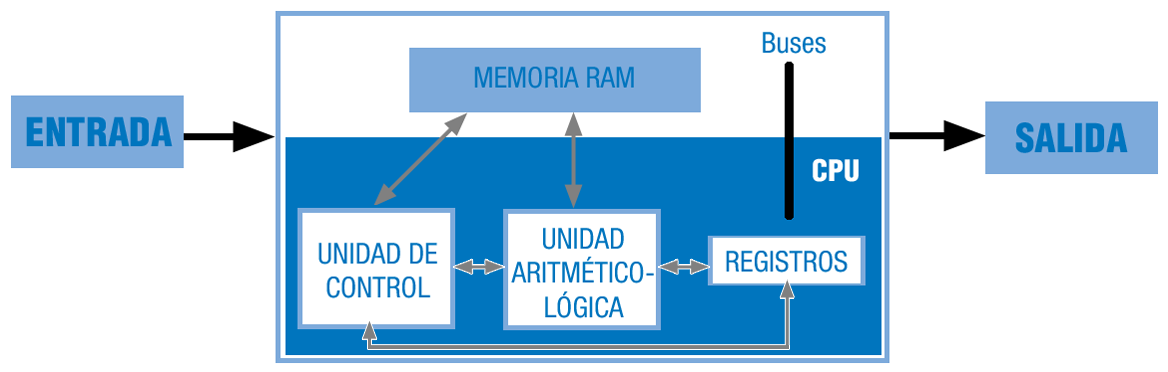
\includegraphics[scale=0.38]{von-neumman.png}
    \caption{Arquitectura John Von Neuman}
\end{figure}

Esta relación software-hardware la podemos analizar desde dos puntos de vista diferentes:

\begin{enumerate}[label={\alph*}]
    \item {\bfseries Desde el punto de vista del sistema operativo}: el sistema operativo es el encargado de coordinar
    el funcionamiento del ordenador, actuando entre este y las aplicaciones que están corriendo en ese momento, gestionando los diferentes recursos hardware que requieren estas aplicaciones (CPU, RAM, interrupciones, dispositivos de E/S..).
    \item {\bfseries Desde el punto de vista de las aplicaciones}: una aplicación solo es un conjunto de programas  escritos en algún lenguaje de programación. Hay multitud de lenguajes de programación, con la característica de que todos están escritos en un idioma que el ser humano puede entender. El hardware por otro lado solo es capaz de interpretar señales eléctricas que se traducen en secuencias de 0 y 1 (código binario). Para que estás aplicaciones puedan ejecutarse en el hardware debe darse un proceso de "traducción" que veremos mas adelante.
\end{enumerate}

\section{Desarrollo de Software}
Entendemos por {\bfseries \gls{Desarrollo de Software}} todo el proceso desde que se concibe la idea hasta que el programa está implementado y funcionando en el ordenador. Aunque en principio pueda parecer una tarea simple, consta de una series de pasos de obligado cumplimiento, pues solo así podemos garantizar que las aplicaciones creadas son eficientes, seguras, fiables y responden a las necesidades de los usuarios finales.

Como veremos más adelante en la unidad, esta serie de pasos se le suele denominar {\bfseries Etapas} en el desarrollo de software. Según el orden y la forma en la que se llevan a cabo estas etapas hablaremos de diferentes ciclos de vida del software. \\

\begin{figure}[h]
    \centering
    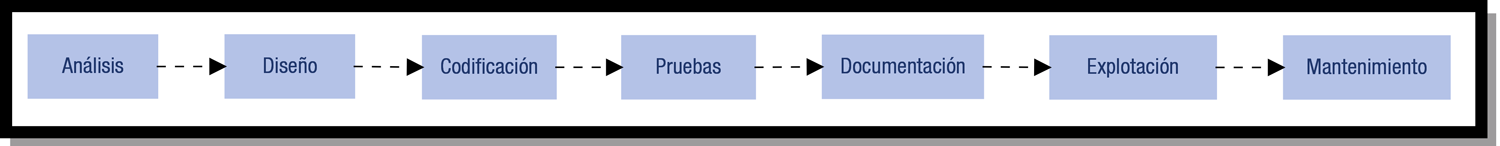
\includegraphics[scale=0.8]{etapas-desarrollo.png}
    \caption{Etapas del Desarrollo de Software}
\end{figure}

Cabe destacar que la construcción de software es un proceso muy complejo y que requiere de una gran coordinación y disciplina del grupo de trabajo que lo desarrolle.

\subsection{Ciclos de Vida del Software}
Ya hemos visto que para crear software debemos seguir un número de pasos conocidos como ciclo de vida del software. Más adelante en esta unidad veremos en que consiste cada paso mas detalladamente. Por ahora, vamos a centrarnos en ver los diferentes ciclos de vida del software que existen atendiendo a como se desarrollan dichos pasos.

Aunque podemos encontrar diferentes clasificaciones sobre los distintos tipos de ciclos de vida del software los mas conocidos y utilizados son los siguientes:

\begin{enumerate}
    \item {\bfseries Modelo en Cascada}: es el modelo de vida clásico del software. Actualmente es prácticamente imposible de utilizar, salvo para desarrollos muy pequeños, ya que es necesario conocer todos los requisitos con antelación y las etapas pasan de una a otra sin retorno, presuponiendo que no ha habido errores en la etapa anterior.
    \item {\bfseries Modelo en Cascada con Realimentación}: es uno de los modelos más utilizados. Proviene del modelo anterior, pero se introduce una realimentación entre etapas, permitiendo que podamos volver hacia atrás en cualquier momento para corregir, depurar o modificar algún aspecto. Es el modelo perfecto si el proyecto es es rígido (pocos cambios y poco evolutivo) y los requisitos están claros. No obstante, si se prevén muchos cambios durante el desarrollo no es el modelo más idóneo.
    \item {\bfseries Modelos Evolutivos}: son los modelos más modernos y tienen en cuenta el aspecto cambiante y evolutivo del software. Dentro de este modulo podemos encontrar dos variantes:
    \begin{enumerate}[label*=\arabic*.]
        \item {\bfseries Modelo Iterativo Incremental}: ésta basado en el modelo en cascada con realimentación, donde las fases se repiten y refinan, propagando su mejora a las fases siguientes. El proyecto se realiza en pequeñas porciones ({\bfseries incrementa}) en sucesivas iteraciones ({\bfseries sprints}) al final de las cuales se ve lo que se ha desarrollado, pudiendo hacer correcciones o modificaciones antes de la siguiente iteración o incluso añadir nuevos requerimientos ({\bfseries adaptativo}). Cada sprint debe proporcional un resultado completo preparado para entregárselo al clientes.
        \item {\bfseries Modelo en Espiral}: es una combinación del modelo anterior con el modelo en cascada. En éste, el software se va construyendo repetidamente en forma de versiones que son cada vez mejores, debido a que se va incrementando la funcionalidad. Es un modelo muy complejo.
    \end{enumerate}
\end{enumerate}

En la actualidad, la {metodologías de desarrollo ágil}, enmarcadas dentro de los modelos evolutivos, están en auge, y metodologías como {\bfseries \href{https://es.wikipedia.org/wiki/Scrum_(desarrollo_de_software)}{Scrum}}, {\bfseries \href{https://es.wikipedia.org/wiki/Desarrollo_guiado_por_pruebas}{TDD}} o {\bfseries \href{https://es.wikipedia.org/wiki/Desarrollo_guiado_por_comportamiento}{BDD}}, así como metodologías híbridas basadas en estas, se están convirtiendo en el estándar de la industria. \cite{batool01}.

\subsection{Herramientas de Apoyo al Desarrollo De Software}
En la práctica, vamos a contar con un conjunto de herramientas que nos van a facilitar llevar a cabo las diferentes etapas del ciclo de vida de desarrollo, automatizando las tareas, ganando con ello fiabilidad y tiempo, y permitiéndonos centrarnos en los requerimientos del sistema y el análisis del mismo.

Las herramientas {\bfseries \gls{CASE}} son un conjunto de aplicaciones que se usan en el desarrollo de software con el propósito de reducir costes y tiempo de proceso, aumentando la productividad. Estas herramientas pueden ayudarnos prácticamente en cualquier etapa del proceso de desarrollo.

El desarrollo rápido de aplicaciones o {\bfseries \gls{RAD}}, es un proceso de desarrollo de software que comprende el desarrollo iterativo, la construcción de prototipos y el uso de herramientas CASE. Hoy en día se usa para referirnos al desarrollo rápido de interfaces de usuario o entornos de desarrollo integrados ({\bfseries \gls{IDE}}) completos.

La tecnología CASE trata de automatizar el proceso de desarrollo para que mejore las calidad del proceso y el resultado final. En concreto, estas herramientas permiten:

\begin{itemize}
    \item Mejorar la planificación del proyecto.
    \item Darle agilidad al proceso.
    \item Generar software mas reutilizable.
    \item Creación de aplicaciones más estandarizadas.
    \item Mejorar las tareas de mantenimiento de las aplicaciones.
    \item Permiten visualizar todo proceso de desarrollo de forma gráfica.
\end{itemize}

Las herramientas CASE se pueden clasificar según su funcionalidad o la función que desempeñan dentro del proceso de desarrollo.

Atendiendo a la función que desempeñan en cada fase del proceso, las herramientas CASE pueden ser:

\begin{itemize}
    \item {\bfseries U-CASE}: ofrecen ayuda en las fases de planificación y análisis de requisitos.
    \item {\bfseries M-CASE}: ofrecen ayuda en el análisis y diseño.
    \item {\bfseries L-CASE}: ofrecen ayuda en la programación del software, detección de errores en código, depuración de programas y pruebas, y en la generación de la documentación.
\end{itemize}

Si tenemos en cuenta su funcionalidad, se pueden diferenciar algunas como:

\begin{itemize}
    \item Herramientas de generación semiautomáticas de código.
    \item Editores {\bfseries \gls{UML}}.
    \item Herramientas de refactorización de código.
    \item Herramientas de mantenimiento, como los sistemas de control de versiones.
\end{itemize}

Algunos ejemplos de herramientas {\bfseries CASE libres} son: ArgoUML, Use Case Maker, ObjectBuilder,...

\section{Lenguajes de Programación}
Podemos definir un \textbf{lenguaje de programación} como un idioma creado artificialmente, que se compone de un conjunto de símbolos y normas que se aplican sobre un alfabeto para obtener un código que el hardware de la computadora pueda entender y procesar. Es el instrumento que tenemos para que el ordenador realice las tareas que necesitamos, dicho de otra forma.

Hay multitud de lenguajes cada uno con su estructura y símbolos. Además cada lenguaje está enfocado en la realización de tareas o áreas determinadas. Por ello, es muy importante la elección del lenguajes o lenguajes de programación en un proyecto.

Los lenguajes de programación han ido evolucionando a través de la historia, podemos ver esta evolución de forma simplificada en la siguientes figura:

\begin{figure}[ht]
    \centering
    
\includegraphics[scale=0.50]{evolucion-lenguajes.png}
    \caption{Evolución de los lenguajes de programación}
\end{figure}

Las principales características de estos lenguajes de son las siguientes:

\begin{itemize}
    \item \textbf{Lenguajes Máquina}:
    \begin{itemize}
        \item Sus instrucciones están compuestas por unos y ceros.
        \item Es el único lenguaje que entiende el ordenador, no necesita traducción.
        \item Fue el primer lenguaje utilizado.
        \item Es único para cada procesador, es decir, no es portable de un equipo a otro.
        \item Hoy en día nadie lo usa.
    \end{itemize}
    \item \textbf{Lenguaje Ensamblador}:
    \begin{itemize}
        \item Sustituyó el lenguaje máquina para facilitar la programación.
        \item Se programa usando mnemotécnicos (instrucciones complejas).
        \item Necesita traducción al lenguaje máquina para poder ejecutarse.
        \item Sus instrucciones hacen referencia a la ubicación física de los archivos y registros.
        \item Es difícil de utilizar.
    \end{itemize}
    \item \textbf{Lenguajes de alto nivel}:
    \begin{itemize}
        \item Sustituyeron al ensamblador para facilitar la programación.
        \item Se utilizan sentencias y órdenes derivadas el inglés. Necesita traducción al lenguaje máquina.
        \item Son más cercanos al razonamiento humano.
        \item Son los más utilizados hoy en día.
    \end{itemize}
    \item \textbf{Lenguajes Visuales}:
    \begin{itemize}
        \item Están sustituyendo a los lenguajes de alto nivel basados en código.
        \item Se programa gráficamente usando y diseñando directamente la apariencia del software.
        \item Su correspondiente código se genera automáticamente.
        \item Necesitan traducción al lenguaje máquina.
        \item Son completamente portables de un equipo a otro.
    \end{itemize}
\end{itemize}

\subsection{Concepto y Características}
Como ya hemos dicho, un \textbf{lenguaje de programación} es un lenguaje formal que le proporciona a una persona, en este caso el programador, la capacidad de escribir una serie de \textbf{instrucciones} o secuencia de órdenes en forma de algoritmo con el fin de controlar el comportamiento ĺógico o físico de un sistema informático, de manera que se pueden obtener diferentes formas de dato o realizar tareas. \cite{lenguaje}

Un lenguaje de programación esta compuesto por:
\begin{itemize}
    \item \textbf{Alfabeto}: conjunto de símbolos permitidos.
    \item \textbf{Sintaxis}: normas de construcción para los símbolos del lenguaje.
    \item \textbf{Semántica}: significado de las construcciones para realizar acciones válidas.
\end{itemize}

Los lenguajes de programación se pueden clasificar de varias formas en base de distintas características:

\begin{itemize}
    \item \textbf{Según lo cercano que este al lenguaje humano}:
    \begin{itemize}
        \item \textbf{Lenguajes de Alto Nivel}: son lenguajes que por su esencia, son mas cercanos al razonamiento humano.
        \item \textbf{Lenguajes de Bajo Nivel}: estos lenguajes están mas próximos al lenguaje que entiende el computador. Los principales son: \textbf{Ensamblador} y \textbf{Lenguaje Máquina}.
    \end{itemize}
    \item \textbf{Según la Técnica de Programación}:
    \begin{itemize}
        \item \textbf{Lenguajes de Programación Estructurados}: usan la técnica de programación estructurada. Ejemplos son Pascal, C, etc...
        \item \textbf{Lenguajes de Programación Orientada a Objetos}: usan las técnica de programación orientada a objetos. Ejemplos son Java, Ruby, Ada, C++, etc...
        \item \textbf{Lenguajes de Programación Funcional}: basan su técnica en el uso de verdaderas funciones matemáticas. Ejemplos son Haskell, Elixir, etc...
        \item \textbf{Lenguajes de Programación Visual}: basados en las técnicas anteriores, permiten programar gráficamente, generando automáticamente el código correspondiente. Ejemplos son Visual Basic.Net, Borland, etc..
    \end{itemize}
\end{itemize}

A pesar de la cantidad de lenguajes de programación que existen, Python, C, Java, C++, C\#, Visual Basic y Javascript, concentran alrededor del 60\% del interés de la comunidad mundial de programadores \cite{tiobe}, aunque en última instancia, la \textbf{elección del lenguaje de programación} para un proyecto dependerá de las características del problema a resolver.

\subsection{Lenguajes de Programación Estructurados}
Los lenguajes estructurados fueron los primeros lenguajes de alto nivel que surgieron, y a partir de ellos, se evolucionó a los diferentes tipos de lenguajes que tenemos hoy en día.

La \textbf{programación estructurada} se define como la técnica para escribir lenguajes de programación que solo permite el uso de tres estructuras de control:

\begin{itemize}
    \item Sentencias secuencias.
    \item Sentencias selectivas (condicionales).
    \item Sentencias iterativas (bucles).
\end{itemize}

Los lenguajes de programación que se basan en este estilo de programación se conocen como \textbf{lenguajes de programación estructurados}.

La programación estructurada fue un gran éxito debido a su sencillez a la hora de construir y leer programas. Aunque como todo, tiene sus ventajas e inconvenientes, que son los siguientes:

\begin{itemize}
    \item \textbf{Ventajas}:
    \begin{itemize}
        \item Los programas son fáciles de leer, sencillos y rápidos.
        \item El mantenimiento de los programas se simplifica.
        \item La estructura del programa es sencilla y clara
    \end{itemize}
    \item \textbf{Inconvenientes}:
    \begin{itemize}
        \item Todo el programa se concentra en un único bloque, si el código crece mucho se hace complejo de manejar.
        \item No permite la reutilización de código, ya que todo el programa va en el mismo bloque.
    \end{itemize}
\end{itemize}

Debido a estos inconvenientes, la \textbf{programación estructurada} evolucionó hacia la \textbf{programación modular}, que divide el programa en trozos de código llamados módulos, con una funcionalidad concreta, y que permiten su reutilización en otras aplicaciones.

Algunos de los lenguajes estructurados mas usados son C, FORTRAN, Pascal, etc...

\subsection{Lenguajes de Programación Orientados a Objetos}
Los \textbf{lenguajes de programación orientados a objetos} tratan los programas, no como un conjunto de instrucciones secuenciales, sino como un \textbf{conjunto de objetos} independientes, que interactúan entre sí, y que son altamente reutilizables en otras aplicaciones.

Su \textbf{principal desventaja} es que no es un paradigma de programación tan intuitivo como la programación estructurada. A pesar de ello, alrededor del 55\% del software que se produce emplea esta técnica. Esto es debido principalmente a que el código es \textbf{muy reutilizable} y a la facilidad de \textbf{depuración}.

Las principales \textbf{características} de estos lenguajes son:

\begin{itemize}
    \item Los objetos del programa tendrán una serie de atributos que los diferencias unos de otros.
    \item Se definen clases como una colección de objetos con características similares.
    \item Mediante los llamados métodos, los objetos se comunican con otros produciendo un cambio de estado.
    \item Los objetos son unidades independientes e indivisibles que forma la base de este paradigma de programación.
\end{itemize}

Algunos de los lenguajes orientados a objetos más utilizados son C++, Java, Ruby, Delphi, etc..

\section{Fases del Desarrollo de Software}
Como hemos visto en puntos anteriores, podemos elegir entre diferentes modelos de desarrollo de software, pero independientemente de cual elijamos, siempre hay un número de etapas que debemos seguir. Estas etapas son las siguientes:

\begin{enumerate}
    \item \textbf{Análisis de Requisitos}: en esta etapa se especifican los requisitos funcionales y no funcionales del sistema.
    \item \textbf{Diseño}: se divide el sistema en partes y se determina la función de cada una.
    \item \textbf{Codificación}: se elige un lenguaje de programación y se codifican los programas.
    \item \textbf{Pruebas}: se prueban los programas para detectar errores y depurarlos.
    \item \textbf{Documentación}: se documentan y guarda información de todas las etapas.
    \item \textbf{Explotación}: instalamos, configuramos y ejecutamos la aplicación en los equipos del clientes.
    \item \textbf{Mantenimiento}: se mantiene el contacto con el cliente para actualizar o modificar la aplicación.
\end{enumerate}

En los siguientes puntos vamos a ver estas etapas con más detalle.

\subsection{Análisis}
Es la primera fase del proyecto y una de las de mayor importancia, ya que todo lo demás dependerá de lo bien detallada que este esta fase. También es una de las más complicadas, ya que no esta automatizada y dependerá en gran medida del análisis que hagamos del problema a resolver.

En esta fase se especifican los requisitos funcionales y no funcionales de la aplicación. Estos \textbf{requisitos} consisten en:

\begin{enumerate}
    \item \textbf{Requisitos funcionales}: estos requisitos especifican que tendrá que realizar la aplicación, que respuesta dará ante todas las entradas, como se comportará en situaciones inesperadas, etc...
    \item \textbf{Requisitos no funcionales}: estos especifican requisitos como el tiempo de respuesta, legislación aplicable, etc...
\end{enumerate}

Es de vital importancia una \textbf{buena comunicación} entre el \textbf{analista} y el \textbf{cliente} para que los requisitos se puedan especificar con el máximo detalle y adecuados a los deseos del cliente.

La culminación de esta fase es un \textbf{documento ERS} (Especificación de Requisitos del Sistema) donde deben quedar especificado lo siguiente:

\begin{itemize}
    \item La planificación de las reuniones que van a tener lugar.
    \item Relación de los objetivos del cliente y el sistema.
    \item Relación de los objetivos funcionales y no funcionales del sistema.
    \item Relación de objetivos prioritarios y temporalización.
    \item Reconocimiento de requisitos mal planteados, etc...
\end{itemize}

Una vez realizado este documento y con los requisitos especificados y detallados, pasaremos a la siguiente fase, la fase de diseño.

\subsection{Diseño}
En esta segunda fase, el sistema debe dividirse en diferentes partes y establecer que relación habrá entre ellas. Decidir exactamente que hará cada parte. En definitiva, debemos crear un modelo funcional-estructural de los requerimientos del sistema global, para poder dividirlo y afrontarlo por separado.

\begin{figure}[ht]
    \centering
    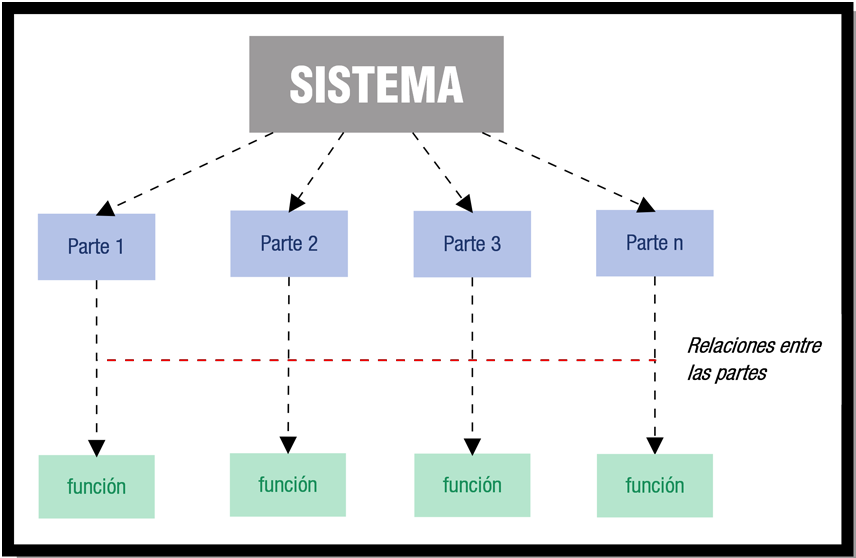
\includegraphics[scale=0.50]{sistema-partes.png}
    \caption{División de la aplicación en partes}
\end{figure}

Además, en esta etapa se deben tomar decisiones que van a afectar el desarrollo del software, como:

\begin{itemize}
    \item Entidades y relaciones de la base de datos.
    \item Selección del lenguaje de programación que se va a utilizar.
    \item Selección del SGBD.
    \item Definición de diagrama de clases.
    \item Definición de diagrama de colaboración.
    \item Definición del diagrama de paso de mensajes.
\end{itemize}

\subsection{Codificación}
En esta fase, con el lenguajes de programación elegido, codificar toda la información anterior y llevarla a código fuente. Esta tarea la realiza el \textbf{programador} y tiene que cumplir con todos los requisitos y restricciones impuestos en la fase de análisis y diseño de la aplicación.

Ademas, el \textbf{código} deberá cumplir con las siguientes \textbf{características}:
\begin{itemize}
    \item \textbf{Modularidad}: que este divido en trozos pequeños funcionales.
    \item \textbf{Corrección}: que haga lo que se pide realmente.
    \item \textbf{Fácil de leer}: que sea fácil de leer y comprender para facilitar su desarrollo y mantenimiento.
    \item \textbf{Eficiencia}: que haga un buen uso de los recursos.
    \item \textbf{Portabilidad}: que se pueda ejecutar en cualquier equipo.
\end{itemize}

El código pasará por un número de fases desde su implementación hasta que se pueda ejecutar. Estas fases son las siguientes:

\begin{enumerate}
    \item \textbf{Código Fuente}: es el código escrito por los programadores usando algún edito o IDE. Se escribe usando algún lenguaje de programación de alto nivel y contiene el conjunto de instrucciones necesaria.
    \item \textbf{Código Objeto}: es el código binario resultado de compilar el código fuente. La \textbf{compilación} es la traducción de una sola vez del programa y se realiza utilizando un compilador. La \textbf{traducción} es la interpretación y ejecución simultánea de un programa línea a línea.
    \item \textbf{Código Ejecutable}: es el resultado de enlazar el código objeto con ciertas \textbf{\gls{rutina}} y \textbf{\gls{biblioteca}} necesarias. El sistema operativo se encarga de cargar el programa en la memoria RAM y proceder a ejecutarlo.
\end{enumerate}

En el \textbf{anexo A.2} también podemos consultar información sobre las máquinas virtuales, que son empleadas en esta etapa del desarrollo con diferentes propósitos.

\subsubsection{Código Fuente}

El código fuente es el conjunto de instrucciones que la computadora debe realizar, escritas por un programador en algún lenguaje de programación. Este conjunto de instrucciones no es directamente interpretable por la máquina, sino que deberá de pasar por un proceso de traducción para que pueda ser ejecutado.

Una parte importante de esta fase es la \textbf{elaboración de un algoritmo}, que definimos como un conjunto de pasos a seguir para obtener la solución a un problema. El algoritmo los diseñamos en pseudocódigo, y con el la codificación a un lenguaje de programación determinado será más rápida y directa.

Para obtener el código fuente de una aplicación se deben seguir estos pasos:
\begin{enumerate}
    \item Se debe partir de la etapa anterior de análisis y diseño.
    \item Se diseñara un algoritmo que simbolice los pasos a seguir para solucionar el problema.
    \item Se elegirá un lenguaje de algo nivel apropiado para las características del software que se quiere codificar.
    \item Se procederá a codificación del algoritmo diseñado.
\end{enumerate}

La culminación de este proceso es la obtención de un documento con todos los \textbf{módulos}, \textbf{funciones}, \textbf{bibliotecas} y \textbf{procedimientos} necesarios para codificar la aplicación. Puesto que el código es inteligible por la máquina habrá que traducirlo, obteniendo así un código equivalente pero ya entendible por el ordenador.

También hay que tener en cuenta, en este punto, bajo que \textbf{licencia} vamos a crear el código, siendo las dos más comunes:

\begin{itemize}
    \item \textbf{Licencias de Código Fuente Abierto}: son licencias que permiten que cualquier usuario o programador pueda estudiar el código, modificarlo y reutilizarlo.
    \item \textbf{Licencias de Código Fuente Cerrado}: estas licencias no dan permisos para editar ni modificar el código fuente.
\end{itemize}

\subsubsection{Código Objeto}
El código objeto es un código intermedio, traducido a unos y ceros, pero que aún no puede ser ejecutado directamente. Consiste en \textbf{bytecode} que esta distribuido en varios archivos, según la cantidad de módulos de software que compongan la aplicación. Este código se \textbf{debe generar} cuando el \textbf{código fuente} este \textbf{libre de errores} sintácticos y semánticos.

El proceso de transformación del código fuente a código puede realizarse de \textbf{dos formas}:
\begin{itemize}
    \item \textbf{Compilación}: el proceso de traducción se realiza sobre todo el programa de una vez. El software que realiza esta operación se llama \textbf{compilador}.
    \item \textbf{Traducción}: el proceso de traducción del código fuente se realiza línea y línea y se ejecuta simultáneamente. No existe código objeto intermedio. El software utilizado se denomina  \textbf{intérprete}. El proceso de traducción es más lento que el de compilación.
\end{itemize}

\subsubsection{Ejecutable}
El código ejecutable es el que obtenemos al enlazar el código objeto con las librerías y rutinas necesarias, resultando un único archivo que puede ser directamente ejecutado por la computadora. Este archivo es ejecutado y controlado por el sistema operativo.

Para obtener un solo archivo ejecutable habrá que enlazar todos los archivos de código objeto mediante una aplicación denominada \textbf{linker} (enlazador) y obtener así un único archivo que ya si es ejecutable directamente por la computadora.

En la siguiente figura vemos el proceso completo para generar archivos ejecutables.

\begin{figure}[ht]
    \centering
    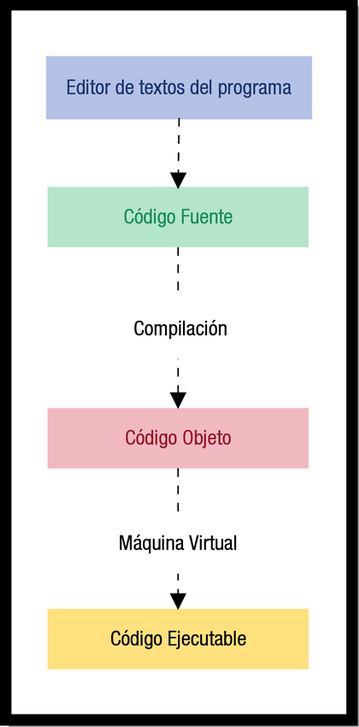
\includegraphics[scale=0.45]{codigo-ejecutable.png}
    \caption{Generación de código ejecutable}
\end{figure}

\subsection{Pruebas}
Una vez obtenido el software, la siguiente fase del ciclo de vida es la realización de pruebas. Normalmente, estás se realizan sobre un conjunto de datos de prueba, que consiste en un conjunto de datos límite  a los que la aplicación es sometida.

La \textbf{realización de pruebas} es una fase \textbf{imprescindible} para asegurar la \textbf{validación} y \textbf{verificación} del software desarrollado y podemos clasificarlas en dos tipos:

\begin{itemize}
    \item \textbf{Pruebas Unitarias}: consiste en probar una a una las diferentes partes del software y comprobar su funcionamiento de forma individual. Un ejemplo de librerías para realizar este tipo de pruebas es \textbf{JUnit} para el lenguaje Java o \textbf{Jest} para Javascript.
    \item \textbf{Pruebas de Integración}: se realiza una vez que se han realizado las pruebas unitarias y consistirán en probar el funcionamiento del sistema completo, con todas sus partes interrelacionadas.
\end{itemize}

La prueba final, también conocida como \textbf{Beta Test} se realizará sobre el entorno de producción del cliente.

\subsection{Documentación}
Para proporcionar toda la información posible sobre el uso del software, tanto a los usuarios como a otros desarrolladores, es necesario crear la \textbf{documentación} de la aplicación.

Debemos ir documentando cada fase del proyecto, ademas, para ir pasando de una otra de forma clara y definida. Una correcta documentación facilitará la reutilización de parte del software para futuros proyectos así como el mantenimiento y su utilización por otros desarrolladores. En la siguiente figura se muestra una tabla con los diferentes tipos de documentación que se pueden generar.

\begin{figure}[ht]
    \centering
    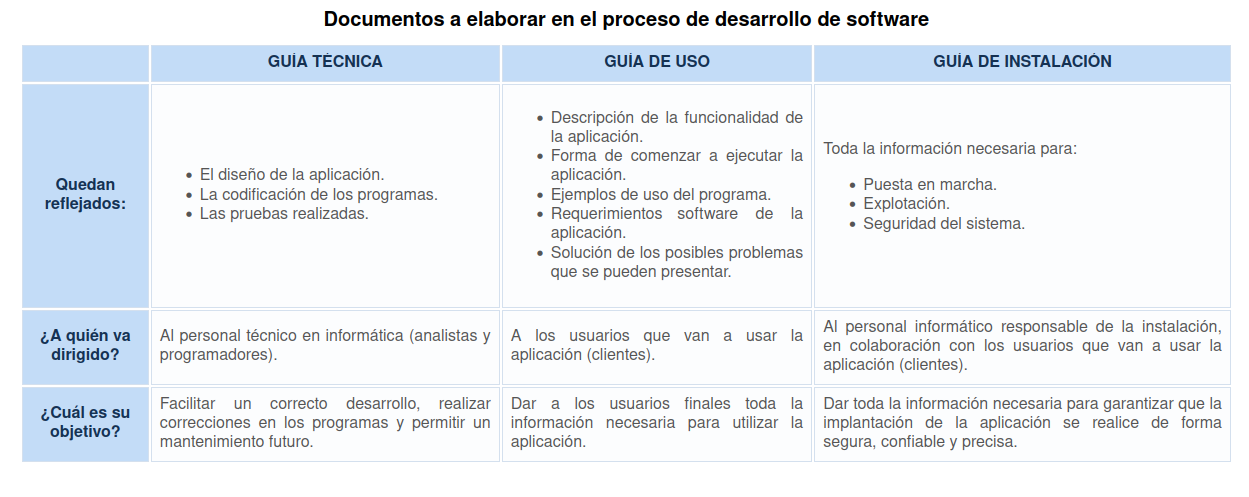
\includegraphics[scale=0.50]{tipos-documentacion.png}
    \caption{Tipos de documentación en el desarrollo de software}
\end{figure}

\subsection{Explotación}
La explotación es la fase en la que los usuarios finales conocen la aplicación y comienzan a utilizarla. Consiste en la instalación, puesta a punto y funcionamiento de la aplicación en el sistema del cliente. Los pasos que se siguen son los siguientes:

\begin{itemize}
    \item En el proceso de \textbf{instalación}, los programas son transferidos al ordenador del cliente, o a un servidor, y posteriormente verificados y configurados. Es importante que el cliente este presente en esta fase para ir comentándole como se realiza la instalación. En este momento, es cuando se suelen realizar las Beta Test.

    \item Ahora pasamos a la fase de \textbf{configuración}, en la que se asignan los parámetros de funcionamiento de la empresa a la aplicación y comprobamos que es operativa. También es probable que la configuración la realicen los usuarios finales, si le hemos proporcionado una guía y de instalación. Si la aplicación es lo suficientemente simple, se puede programar la configuración para que se realice de forma automática.

    \item Una vez configurado, se pasa a la fase de \textbf{producción}, donde la aplicación pasa a manos del cliente y se da comienzo a la explotación del software.
\end{itemize}

Es muy importante tener todo preparado antes de presentar el producto final al cliente, ya que esta es una de las fases mas críticas del proyecto.

\subsection{Mantenimiento}
El software es cambiante y deberá actualizarse y evolucionar con el tiempo. Deberá adaptarse a las mejoras de hardware del mercado y afrontar situaciones que no estaban prevista cuando se creó. Además, siempre pueden surgir errores que deberán irse corrigiendo y nuevas versiones del producto mejores que la anterior. Por todo ello se pacta un servicio de mantenimiento del sistema con el cliente, que tendrá un coste temporal y económico.

El \textbf{mantenimiento} se define como el proceso de control, mejora y optimización del software. Su duración es la mayor de todo el ciclo de vida del software, ya que también comprende las actualizaciones y evoluciones futuras del mismo.

Los tipos de cambios que se pueden realizar en una aplicación son los siguientes:

\begin{itemize}
    \item \textbf{Perfectivos}: se realizan para mejorar la funcionalidad del software.
    \item \textbf{Evolutivos}: en el futuro el cliente tendrá nuevas necesidades, por lo que se requerirán nuevas modificaciones, expansiones o eliminación de código.
    \item \textbf{Adaptativos}: modificación y actualizaciones para adaptarse a las nuevas tendencias del mercado, como nuevo hardware, nuevos frameworks, etc...
    \item \textbf{Correctivos}: son los que se realizan para la corrección de errores.
\end{itemize}

Si quieres ampliar información sobre las fases de desarrollo, en \href{http://profayadira.yolasite.com/resources/Roles_desarrollo_software.pdf}{este documento} se detallan los diferentes roles que podemos encontrar en el proceso de desarrollo y que funciones tienen dentro de este, así como sus interacciones.

\section{Entornos de Desarrollo}
En esta sección vamos a hablar de los entornos de desarrollo, herramientas que nos en la fase de codificación a la hora de programar nuestras aplicaciones.

En muchas ocasiones, las personas que empiezan a programar lo hacen usando un \textbf{editor simple}, un \textbf{compilador} y un \textbf{depurador}. Pero la mayoría de gente acaba usando un algún entorno de desarrollo integrado o IDE (Integrated Development Environment) para crear las aplicaciones.

Un \textbf{entorno de desarrollo integrado} (IDE), es un tipo de software compuesto por un conjuntos de herramientas que nos facilitan el proceso de programación. Estas herramientas suelen ser:

\begin{itemize}
    \item \textbf{Editor} de código de programación.
    \item \textbf{Compilador}.
    \item \textbf{Intérprete}.
    \item \textbf{Depurador}.
    \item \textbf{Constructor de interfaz} gráfico.
\end{itemize}

Los primeros IDEs nacieron a principios de los años 70, pero fue en la década de los 90 cuando se popularizaron. Su objetivo principal es ganar fiabilidad y tiempo en los proyectos de software, proporcionando una serie de componentes bajo una misma interfaz gráfica, con la consiguiente comodidad, aumento de eficiencia y reducción del tiempo de codificación.

En un primer momento los IDEs estaban enfocados en un lenguaje de programación concreto, pero actualmente suelen soportar diferentes lenguajes de programación, algunos de forma predeterminada y otros mediante la instalación de plugins. Algunos ejemplos son Eclipse, Netbeans, VS Code, Intellij Idea, etc..

En este tema nos vamos a centrar en la instalación de \textbf{Netbeans} en Ubuntu y veremos como se configurar y se generan ejecutables, haciendo uso de sus componentes y herramientas.

\subsection{Evolución Histórica}
En la época de utilización de las \textbf{\gls{tarjetas perforadas}} como sistema de almacenamiento los \textbf{Entornos de Desarrollo Integrado} sencillamente no tenían sentido. Los programas estaban escritos con \textbf{diagramas de flujo} y entraban al sistema a través de estas tarjetas para posteriormente compilarse.

El primer lenguaje de programación que utilizó un IDE fue BASIC, que fue el primero en abandonar las tarjetas perforadas. Este primer IDE estaba basado exclusivamente en la consola de comandos. Sin embargo, el uso que hacía de la gestión de archivos, compilación y depuración era totalmente compatible con la definición de IDE actual.

A nivel popular, el primer IDE puede considerarse que fue el IDE \textbf{Maestro}. Nació a principios de los años 70 y fue instalado por unos 22.000 programadores en todo el mundo, liderando este campo durante los años 70s y 80s.

El uso de los IDEs se popularizó en los años 90 y hoy en día contamos con una infinidad de IDEs, tanto de licencia libre como propietaria.

\begin{figure}[ht]
    \centering
    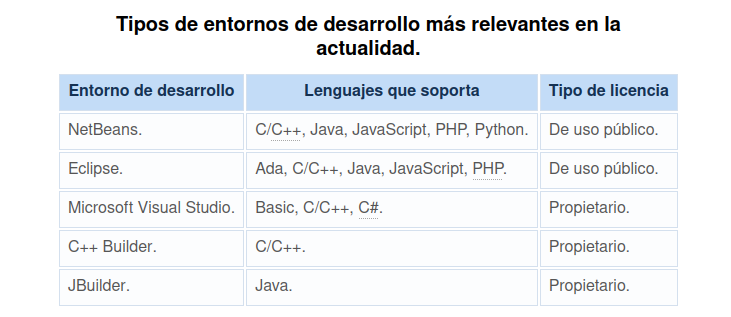
\includegraphics[scale=0.60]{tipos-de-IDE.png}
    \caption{Tipos de IDE actuales}
\end{figure}

\subsection{Funciones de un Entorno de Desarrollo}
En los puntos anteriores ya hemos visto los componente que tiene un IDE, como editor de textos, compilador, depurador, etc... En este punto vamos a ver sus funciones de estos componentes, que se podrían resumir en las siguientes:

\begin{itemize}
    \item \textbf{Editor de código}: resaltado y coloreado de la sintaxis.
    \item \textbf{Autocompletado} de código, atributos, métodos, clases, etc...
    \item Identificación automática de código.
    \item Herramientas de \textbf{concepción visual} para crear y manipular componentes visuales.
    \item \textbf{Asistentes} y utilidades de gestión y \textbf{generación de código}.
    \item Archivos fuentes en unas carpetas y compilación en otras. (estructuración del código)
    \item \textbf{Compilación} de proyectos complejos en \textbf{un solo paso}.
    \item \textbf{Control de versiones}: tener un único almacén de archivos compartido por todos los desarrolladores de un proyectos con mecanismos de seguimiento de cambios, recuperación a un estado anterior, etc...
    \item Soporte \textbf{cambios} de varios usuarios de forma \textbf{simultánea}.
    \item \textbf{Generación de documentación} automática.
    \item \textbf{Detección} de errores de \textbf{sintaxis} en tiempo real.
    \item \textbf{Refactorización de código}: cambios menores en el código que aumentan la legibilidad sin alterar la funcionalidad.
    \item \textbf{Indentación} automática del código para aumentar la legibilidad.
    \item \textbf{Depuración}: seguimiento de variables, puntos de ruptura y mensajes de error del intérprete.
    \item Instalación de \textbf{plugins} y módulos que expanden la funcionalidad del IDE.
    \item \textbf{Administración} de las \textbf{interfaces de usuario}.
    \item \textbf{Administración} de las \textbf{cuentas de usuario}.
\end{itemize}

Como podemos ver en esta larga lista, los IDEs tiene un montón de funcionalidades que nos va a facilitar el proceso de codificación en muchos aspectos. Hoy en día es imprescindible su utilización para mejorar la productividad y centrarlos en la programación, dejando al IDE a cargo de otros aspectos más ``secundarios''.

\subsection{Estructura de un Entorno de Desarrollo}
Como ya hemos comentado, un IDE esta formado por un conjunto de componentes software que determinan sus funciones. Los componente principales que podemos encontrar en un IDE, son los siguientes:

\begin{itemize}
    \item \textbf{Editor de Textos}: resalta y colorea la sintaxis, tiene funciones para autocompletar el código, ayuda y listado de funciones y parámetros, inserción automática de paréntesis o corchetes, tabulaciones y espacios, etc...
    \item \textbf{Compilador/Intérprete}: detección de errores de sintaxis en tiempo real y funciones para la refactoriación.
    \item \textbf{Depurador}: botón de ejecución y traza, puntos de ruptura y seguimiento de variables. Opción de depurar en servidores remotos.
    \item \textbf{Generador automático de herramientas}: para la generación y manipulación de componentes visuales y todo un arsenal de asisten y utilidades de gestión y generación de código.
    \item \textbf{Interfaz Gráfica}: es la interfaz principal del IDE y nos permite usar todas las funcionalidades y utilizar diferentes lenguajes de programación en un mismo IDE, permitiendo el acceso a innumerables bibliotecas y plugins, aumentado las opciones de nuestro programa.
\end{itemize}

\subsection{Entornos Integrados Libres y Propietarios}
Según la licencia que usen los entornos de desarrollo, podemos encontrarnos entornos de desarrollo \textbf{libres} y entornos de desarrollo \textbf{propietarios}. La elección de la licencia del IDE en un proyecto es de vital importancia.

\begin{itemize}
    \item \textbf{Entornos de Desarrollo Libres}

    Son aquellos que usan licencias open source, que permiten que el código del IDE este disponible para cualquier persona. Pueden ser gratuitos. En la siguiente figura se muestran los mas utilizados, aunque falta alguna opción como \textbf{Visual Studio Code} (no confundir con Microsoft Visual Studio, que es la opción propietaria de MS).

    \begin{figure}[ht]
        \centering
        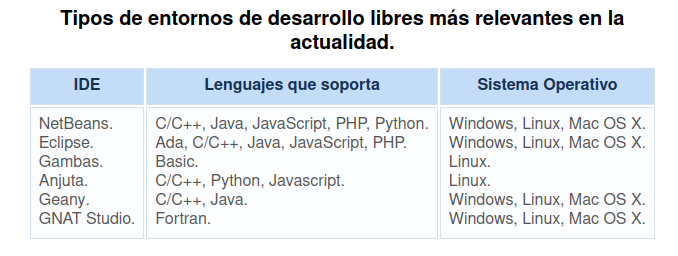
\includegraphics[scale=0.60]{ide-libres.png}
        \caption{IDEs con licencia libre}
    \end{figure}

    \item \textbf{Entornos de Desarrollo Propietarios}

    Son aquellos cuya licencia es propietaria, por lo tanto el código fuente no estará disponible para los usuarios. Se necesita pagar por su uso. En la siguiente figura se muestran algunos ejemplos.

    \begin{figure}[ht]
        \centering
        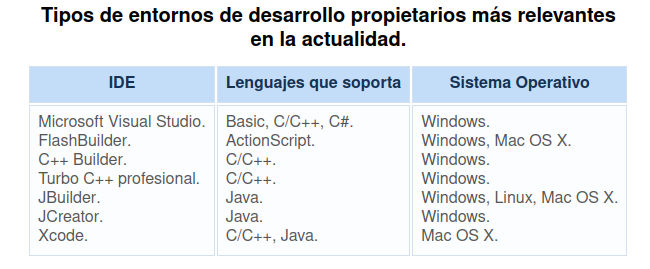
\includegraphics[scale=0.60]{ide-prop.png}
        \caption{Entornos de desarrollo propietarios}
    \end{figure}
\end{itemize}

La elección del entorno de desarrollo así como de su licencia deberá ajustarse al lenguaje de programación que vamos a usar, así como a los requisitos del proyecto.

\section{Conclusiones}
En este tema hemos visto el ciclo de vida de software y la importancia que tiene en el desarrollo de aplicaciones de forma metódica. Algunas etapas tienen más importancia que otras, por ejemplo, si la primera etapa, \textbf{análisis}, no se realiza de forma meticulosa, puede lastrar el resto de etapas y perjudicar el proceso de desarrollo. Por ello, es de suma importancia dedicarle el tiempo necesario a cada etapa. Aunque hay diferentes metodologías de desarrollo, todos tienen las mismas etapas.En la actualidad se están imponiendo \textbf{metodologías de desarrollo ágil}.

Si queremos obtener más información, podemos consultar \href{https://www.itmplatform.com/es/blog/ciclos-de-vida-clasico-iterativo-y-agil/}{este enlace}, donde se nos hace un resumen de las principales metodologías de desarrollo actuales.

Por otro lado hemos visto que es un entorno de desarrollo integrado y como su utilización nos facilita enormemente la programación. La elección que se haga de un entorno u otro dependerá de las preferencias de cada uno, aunque también de los requisitos del proyecto y del lenguaje de programación que vayamos a utilizar. Lo que está claro es que son una herramienta indispensable para cualquier programador.

% Apéndice
\appendix

% Change appendix display options
\titleformat{\chapter}{\bfseries\Huge}{\thechapter.}{1ex}{}

\chapter{Anexos Tema 1}

\section{Secuencias de Control en Programación Estructurada}
En este punto vamos a hacer un breve repaso de las sentencias básicas de control en los lenguajes de programación estructurados.

\begin{itemize}
    \item \textbf{Sentencias Secuenciales}

    Son aquellas sentencias que se ejecutan una detrás de otra.

    \begin{figure}[h]
        \begin{tcolorbox}[sharp corners, colback=yellow!30, colframe=white!20]
            \scriptsize
            \begin{verbatim}

            printf (“declaración de variables”);
            int numero_entero;
            espacio=espacio_inicio + veloc*tiempo;
            \end{verbatim}
        \end{tcolorbox}
        \caption{Sentencias secuenciales en C}
    \end{figure}

     \item \textbf{Sentencias Selectivas} (Condicionales)

     Son aquellas sentencias en las que se evalúa una condición, ejecutándose una serie de instrucción en el caso de que la condición sea verdadera y otras en el caso de que sea falsa.
     Si estructura es la siguiente:

     \begin{figure}[h]
         \begin{tcolorbox}[sharp corners, colback=yellow!30, colframe=white!20]
             \scriptsize
             \begin{verbatim}
              if (condición) then
                instrucciones a ejecutar si es verdadera
              else
                instrucciones a ejecutar si es falsa
             \end{verbatim}
         \end{tcolorbox}
         \caption{Estructura sentencia condicional if}
     \end{figure}

     En la siguiente figura podemos ver un ejemplo básico en el lenguaje de programación C.

     \begin{figure}[h]
         \begin{tcolorbox}[sharp corners, colback=yellow!30, colframe=white!20]
             \scriptsize
             \begin{verbatim}
             if (a >= b)
                c = a - b;
             else
                c = a + b;
             \end{verbatim}
         \end{tcolorbox}
         \caption{Sentencia if en el lenguaje C}
     \end{figure}

     \item \textbf{Sentencias Repetitivas} (iteraciones o bucles)

     Un bucle es una serie de acciones que se ejecutan mientras que se cumpla una condición. Su estructura básica es la siguiente.

     \begin{figure}[h]
         \begin{tcolorbox}[sharp corners, colback=yellow!30, colframe=white!20]
             \scriptsize
             \begin{verbatim}
             // Bucle whle ... do

             while (condición)
                instrucciones a repetir
             done

             // Bucle for

             for (condición_inicial; incremento; condición_de_parada)
                instrucciones a repetir
             \end{verbatim}
         \end{tcolorbox}
         \caption{Documento SGML simple}
     \end{figure}

     En la siguiente figura vemos un ejemplo de un while...do en C, en este lenguaje, la palabra done se omite.

     \begin{figure}[h]
         \begin{tcolorbox}[sharp corners, colback=yellow!30, colframe=white!20]
             \scriptsize
             \begin{verbatim}
             int num;
             num = 0;

             while (num<=10) {
                printf("Repetición numero %d", num);
                num = num + 1;
             };
             \end{verbatim}
         \end{tcolorbox}
         \caption{Documento SGML simple}
     \end{figure}

\end{itemize}

\section{Máquinas Virtuales}
Una máquina virtual es un tipo de software que separa el funcionamiento del ordenador de los componente hardware. Esta capa de software desempeña un papel muy importante en el funcionamiento de los lenguajes de programación, tanto compilados como interpretados.

Con el uso de máquinas virtuales podremos desarrollar y ejecutar código en cualquier equipo, independientemente de las características concretas de los componente físicos de este, garantizando la \textbf{portabilidad} de las aplicaciones.

Las \textbf{funciones} principales de una máquina virtual son las siguientes:

\begin{itemize}
    \item Conseguir que las aplicaciones sean portables.
    \item Reservar memoria para los objetos que se crean y liberar la memoria no utilizada.
    \item Comunicarse con el sistema donde se instala la aplicación (host) para el control de los recursos hardware implicados en el proceso.
    \item Cumplimento de las normas de seguridad de las aplicaciones.
\end{itemize}

Las principales \textbf{características} de estás, son las siguientes:

\begin{itemize}
    \item La máquina virtual \textbf{aísla la aplicación} de los detalles físicos en del equipo en cuestión. Cuando el código se compila se obtiene \textbf{bytecode}. La máquina virtual funciona como una capa de software de bajo nivel y actual de puente entre el bytecode de la aplicación y los dispositivos físicos del sistema.
    \item La máquina virtual \textbf{verifica} todo el bytecode antes de ejecutarlo.
    \item También se encarga de \textbf{proteger} las \textbf{direcciones de memoria}.
\end{itemize}

\subsection{Frameworks}
Un \textbf{framework} es una estructura de ayuda al programador, en base a la cual podemos desarrollar proyectos sin partir desde cero. Se trata de una plataforma de software donde están definidos bibliotecas, programas de soporte, lenguaje interpretado, etc...

Con el uso de frameworks podemos pasar más tiempo analizando los requisitos del sistema y las especificaciones técnicas de nuestra aplicación, ya que la tarea laboriosa de los detalles de programación queda bastante resuelta. Pero como todo, tiene sus ventajas e inconvenientes.

\begin{itemize}
    \item \textbf{Ventajas} de usar un framework:
    \begin{itemize}
        \item \textbf{Desarrollo rápido} de software.
        \item \textbf{Reutilización} de partes de código para otras aplicaciones.
        \item \textbf{Diseño uniforme} del software.
        \item \textbf{Portabilidad} de las aplicaciones de un computador a otro, ya que los bytecode que se generan podrán ser ejecutados en cualquier sobre cualquier máquina virtual.
    \end{itemize}

    \item \textbf{Inconvenientes} de usar un frameworks:
    \begin{itemize}
        \item \textbf{Gran dependencia} del código respecto al framework utilizado.
        \item La instalación y configuración del framework en nuestro equipo \textbf{consume} bastantes \textbf{recursos} del sistema.
    \end{itemize}
\end{itemize}

Algunos ejemplos de frameworks son:

\begin{itemize}
    \item \textbf{.NET}: framework para el desarrollo de aplicaciones sobre Windows. Ofrece el ``Visual Studio .NET'' que nos proporciona facilidades para construir aplicaciones y su motor es el ``.NET Framework'', que permite ejecutar dichas aplicaciones.
    \item \textbf{Java Spring}: son un conjunto de bibliotecas (API's) para el desarrollo y ejecución de aplicaciones. Es uno de los más empleados en Java y es recomendable saber manejarlo.

    Si quieres profundizar más en este framework, puedes consultar los siguientes enlaces:
    \begin{itemize}
        \item \href{https://educacionadistancia.juntadeandalucia.es/formacionprofesional/pluginfile.php/35569/mod/_scorm/content/16/spring_tutorial_v0.271.pdf}{Instalación de Spring e Información Básica}
        \item \href{https://www.uv.es/grimo/teaching/SpringMVCv4PasoAPaso/index.html}{Desarrollando una aplicación Spring Paso a Paso}
    \end{itemize}
\end{itemize}

\subsection{Entornos de Ejecución}
Un entorno de ejecución es un servicio de una máquina virtual que sirve como base de software para la ejecución de aplicaciones. En ocasiones pertenece al propio sistema operativo, pero se puede instalar de forma independiente que funcionará por debajo del programa. Se denomina \textbf{runtime} al tiempo que tarda un programa en ejecutarse en la computadora.

El \textbf{funcionamiento} de un entorno de ejecución se puede resumir en:

\begin{itemize}
    \item El \textbf{entorno de ejecución} esta formado por \textbf{la máquina virtual} y las \textbf{API's} (bibliotecas de la clase estándar, necesarias para que la aplicación pueda ser ejecutada). Estos dos componentes se suelen distribuir conjuntamente, ya que necesitan ser compatibles entre sí.
    \item El entorno actúa como \textbf{intermediario} entre el \textbf{código fuente} y el \textbf{sistema operativo}.
    \item Si lo que queremos es desarrollar nuevas aplicaciones, nos es suficiente con un entorno de ejecución.
    \item Para desarrollar aplicaciones necesitamos algo más, un \textbf{entorno de desarrollo}.
\end{itemize}

\begin{figure}[ht]
    \centering
    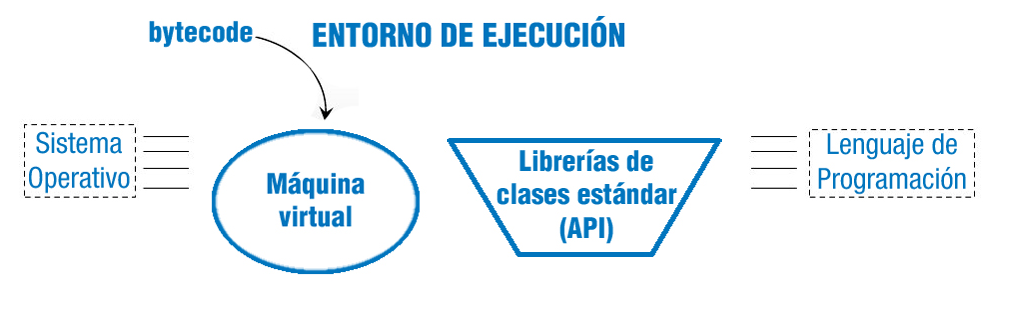
\includegraphics[scale=0.50]{entorno-ejecucion.png}
    \caption{Entorno de Ejecución}
\end{figure}

El entorno de desarrollo, realizará varias funciones durante la ejecución de la aplicación, sus principales funciones durante la \textbf{ejecución} son las siguientes:

\begin{itemize}
    \item Configurar la memoria principal disponible del sistema
    \item Enlazar los archivos del programa con las bibliotecas existentes y subprogramas creados.
    \item Depurar los programas: comprobar la existencia de errores semánticos del lenguaje.
\end{itemize}

\subsection{Java Runtime Environment}
El \textbf{Java Runtime Environment} o \textbf{JRE} es un conjunto de utilidades que permiten la ejecución de aplicaciones Java. Un usuario solo necesita el JRE para ejecutar aplicaciones en Java.\cite{wiki03}

Los \textbf{componentes} principales de JRE son:

\begin{itemize}
    \item La \textbf{Máquina Virtual Java}, que es el componente que interpreta el código de la aplicación escrito en Java.
    \item Bibliotecas de clase estándar que implementan la \textbf{API de Java}.
    \item Las dos anteriores, JVM y API, deben ser consistentes entre ellas.
\end{itemize}

Para instalar JRE, lo primero que debemos hacer es descargarlo. Java es software libre, por lo que podemos descargarlo de forma libre y gratuita. Una vez descargado, solo habrá que seguir los pasos del asistente de instalación. En los siguientes enlaces, podemos ver una guía de instalación detallada:

\begin{itemize}
    \item \href{https://www.java.com/es/download/help/linux_install.html}{Guía de Instalación de Java en Linux}
    \item \href{https://www.java.com/es/download/help/windows_manual_download.html}{Guía de Instalación de Java en Windows}
\end{itemize}



% Glossary

\glsaddall
\printglossaries

% Bibliography

\newpage
\addcontentsline{toc}{chapter}{Bibliografía}
\bibliography{citas}
\bibliographystyle{unsrt}

\end{document}